
\documentclass[11pt,a4paper]{article}
\usepackage[left=2cm,right=2cm,top=2cm,bottom=2cm]{geometry}
\usepackage[utf8]{inputenc}
\usepackage[T1]{fontenc}
\usepackage[english]{babel}
\usepackage{setspace}
\usepackage{parskip}
\usepackage{enumitem}
\usepackage{hyperref}
\usepackage{mathptmx} 
\usepackage{csquotes}
%\usepackage[backend=biber,style=apa]{biblatex}
\usepackage[backend=biber,style=numeric]{biblatex}
\renewcommand*{\bibfont}{\small}  % Schriftgröße der Referenzen
\usepackage{soul} % us hl to highlight
\usepackage{xcolor} % Optional, falls du die Farbe ändern willst
\usepackage[most]{tcolorbox}  % in der Präambel
\usepackage{titlesec}
\usepackage{changepage}
\usepackage{comment}
\usepackage{tabularx}
\usepackage[table]{xcolor} % Optional: für dezente Hintergrundfarben
\usepackage{booktabs}      % Für schönere Tabellenlinien
\usepackage{longtable}
\usepackage{array}
\usepackage[table]{xcolor}
\usepackage{graphicx}   % wichtig fürs Einfügen von Bildern
\usepackage{caption}    % erlaubt auch unnummerierte Captions (optional)
\usepackage{wrapfig}   % Text um Bilder herum
\captionsetup[figure]{name=Fig.}
\captionsetup[figure]{aboveskip=1pt, belowskip=-2ex}
\captionsetup[figure]{font={scriptsize,it}}

% Vor der Tabelle:
\renewcommand{\arraystretch}{1.2}
\rowcolors{2}{gray!10}{white}

\titlespacing*{\section}{0pt}{0.8ex plus 0.5ex minus .2ex}{0.3ex}
\titlespacing*{\subsection}{0pt}{0.8ex plus 0.5ex minus .2ex}{0.3ex}
\titlespacing*{\subsubsection}{0pt}{0.8ex plus 0.5ex minus .2ex}{0.3ex}
\titleformat{\paragraph}[block]{\normalfont\normalsize\bfseries}{\theparagraph}{1em}{}
\titlespacing*{\paragraph}{0pt}{0.5ex plus 0.2ex minus 0.1ex}{1ex}

\sethlcolor{yellow} % Setzt die Highlight-Farbe
\setlist[itemize]{leftmargin=*, topsep=-3pt, itemsep=0pt}
\setstretch{1}

\addbibresource{/Users/sweis/Data/Arbeit/Bibliothek/NewMasterBib_LaTex.bib}

\begin{document}

\hl{Name, institution, and contact details of the applicant (one person only) and a list of the scientists or institutions involved in the research project (max. 2 A4 pages)
CVs and lists of publications need not be submitted.}

PD Dr. rer. medic. Susanne Weis, Heinrich Heine University Düsseldorf; \\
Gruppenleiterin „Variabilität des Gehirns“, Gehirn und Verhalten (INM-7), Institut für Neurowissenschaften und Medizin,  
Forschungszentrum Jülich; \\
E-Mail: S.Weis@fz-juelich.de

Simon

INM-7: The proposed work is embedded in a multidisciplinary working team combining knowledge in the field of neuropsychology, structural and functional MRI analysis, computational neuroscience and machine learning. 

Dr. Kaustubh Patil, head of the working group “Applied Machine Learning”

Rick Betzel is an associate professor at the Psychological and Brain Sciences Department of Psychological and Brain Sciences at Indiana University Bloomington, USA. He is an expert in principles of time-varying functional network reconfiguration and its relationship to ongoing cognitive processes and one of the developers of the edge time series approach which we will employ within the project suggested here. 


\newpage

\section*{\Large\textbf{Dynamic Cognition: Movies as a Window into Sex Differences in the Brain}}
\hfill

\subsection*{Project Description} 
\subsection*{Background and Research Question} 

Functional brain imaging techniques, in particular fMRI have been widely used to investigate sex differences in the brain.
Such differences in structural and functional brain organization play a crucial role in healthy human brain development, 
aging, as well as the manifestation of psychiatric and neurological disorders \parencite{cahillWhySexMatters2006a,gobinathSexHormonesGenotype2017a}. 
Consequently, an understanding of sex differences in the human brain and 
their underlying mechanisms is critical for understanding both normative behavior and psychopathology. \\
In the present proposal, we aim to employ novel brain imaging methodology utilizing naturalistic viewing (NV), 
i.e. watching of Hollywood movies clips in the scanner, to broaden our knowledge of sex differences in the brain. 
While it is common knowledge that women and men often react differently to complex scenarios in 
films - think of how a couple might debate a movie's emotional impact after leaving the cinema - our study 
delves deeper than these everyday observations. Instead of relying on stereotypes such as 
'women like emotional scenes, men like action', we will analyze in detail how brain activity and functional 
connectivity (FC) differs when women and men watch various movie scenes. This could reveal, for example, 
that women process subtle social cues in dialogues differently from men, while men might react more strongly to 
visual hints in action scenes that foreshadow danger. Through a thorough analysis of females' and males' brain 
responses to a variety of different movie scenes, we aim to develop a well-founded understanding of cognitive 
sex differences that advances our knowledge of sex differences in brain function beyond 
the current state of research.\\
So far, our understanding of sex differences in the brain is still far from complete. 
While there is some agreement on the existence of sex differences in specific cognitive domains like 
language and spatial processing, some researchers argue that female and male brains are altogether more similar 
than different \parencite{joelSexGenitaliaHuman2015a} and that the overlap between the sexes is larger than their differences. 
Importantly, neuroimaging research on sex difference has so far only been able to capture certain aspects of these 
differences.\\ 
Classically, sex differences in the brain have been studied using task-based (TB) fMRI with tightly 
controlled tasks, offering insights limited to specific cognitive domains 
(e.g. \parencite{thimmMenstrualCycleEffects2014a,weisDynamicChangesFunctional2011,weisEstradiolModulatesFunctional2008}. 
However, due to the highly 
controlled and artificial nature of the tasks, ecological validity of task-related fMRI is usually 
very low and does not reflect cognitive sex differences as observed in daily life. More recently, 
resting state (RS) approaches have been employed, in which fMRI data is acquired while subjects relax 
in the scanner without any specific task demand or visual or auditory stimulation. Earlier
RS studies examined group differences in connectivity patterns between women and men. 
More recently, however, machine learning (ML) methods have been applied to move beyond group averages: sex classification approaches 
use RS data to predict the sex of individual subjects 
\begin{wrapfigure}{r}{0.3\textwidth} % r = rechts, l = links
  \vspace{-10pt} % optional: kleine Korrektur, damit es bündig startet
  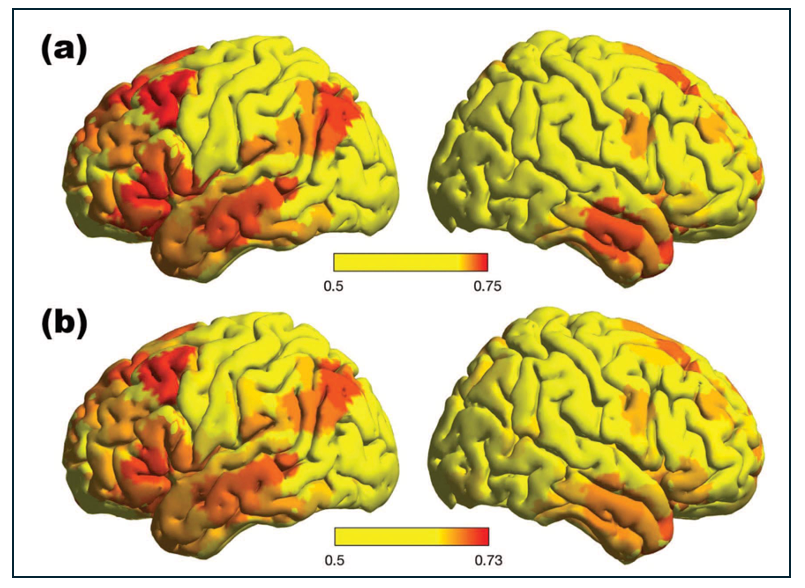
\includegraphics[width=\linewidth]{sex_classification.png}
  \caption{ROI-based sex classification shows high accuracies for (a) within sample CV and (b) across sample classification.}
  \label{fig:sexclass}
\end{wrapfigure}
and then infer which brain networks contribute most to 
distinguishing females from males. Using such an ML approach, we identified regionally specific brain networks 
that support successful classification, which, importantly, generalized from a training sample to an independent 
sample and revealed that predictive power—and thus cognitive sex differences—are most pronounced in higher-level 
cognitive regions involved in language, social cognition, and emotion processing 
\parencite{weisSexClassificationResting2020a,wierschAccurateSexPrediction2023a,wierschSexDifferencesBrain2021a}.
\par\vspace{-1\parskip}\noindent
Importantly though, RS fMRI only reflects the brain in a specific state, which has commonly interpreted as 
intrinsic brain organization and thus constitutes a trait rather than a state. Moreover, while a state of free mind wandering happens often in real life, what remains largely unexplored are sex differences in the “brain in action”, i.e. when encountering complex, multimodal stimulation resembling real-life experiences.
The present proposal aims to contribute to closing this gap in knowledge by applying the newly 
emerging NV approach to examine sex-specific brain responses in ecologically valid contexts. NV focuses on 
cognitive processes in dynamic, temporally extended, naturalistic contexts, which are much more akin to
situations which the brain must deal with in real life. In NV tasks, participants in the scanner are 
presented with naturalistic material like movies. For the participants, there is no other task demand rather 
than watching the clips. NV offers an engaging task for the subject and thus avoids boredom in the scanner. 
Importantly, as opposed to RS, all participants are exposed to the same stimulus, for which content and timing 
is known and can be used in the analyses. NV approaches offer complex, dynamic and ongoing stimulation similar 
to experiences in everyday situations, where low-level (audiovisual) and high-level (cognitive and emotional) 
content vary fluidly, creating a multimodal and immersive experience \parencite{sonkusareNaturalisticStimuliNeuroscience2019}, offering the 
opportunity to capture dynamic neural processing in ecologically valid contexts \parencite{vanderwalMoviesMagnetNaturalistic2019}. 
Furthermore, NV has been shown to improve reliability and individual identifiability over RS \parencite{krollNaturalisticViewingIncreases2023} 
with a recent study from our lab \parencite{krollNaturalisticViewingIncreases2023} showing that the use of NV enhances the detection of 
FC patterns that are unique at the individual level.\\ 
Our lab pioneered NV analysis methods. We recently developed the topography-based predictive framework 
(TOPF) \parencite{liTopographybasedPredictiveFramework2023a}, which identifies individual-specific evoked activity topographies in a data-driven 
manner and examines their behavioural relevance using a ML predictive framework. 
TOPF effectively and stably captures individual differences in evoked brain activity and successfully predicts phenotypes across 
cognition, emotion and personality, and will be employed in the present context to uncover differences between 
females and males. In preliminary work using TOPF \parencite{liTopographybasedPredictiveFramework2023a} on NV data, we 
\begin{wrapfigure}{r}{0.3\textwidth} % r = rechts, l = links
  \vspace{-10pt} % optional: kleine Korrektur, damit es bündig startet
  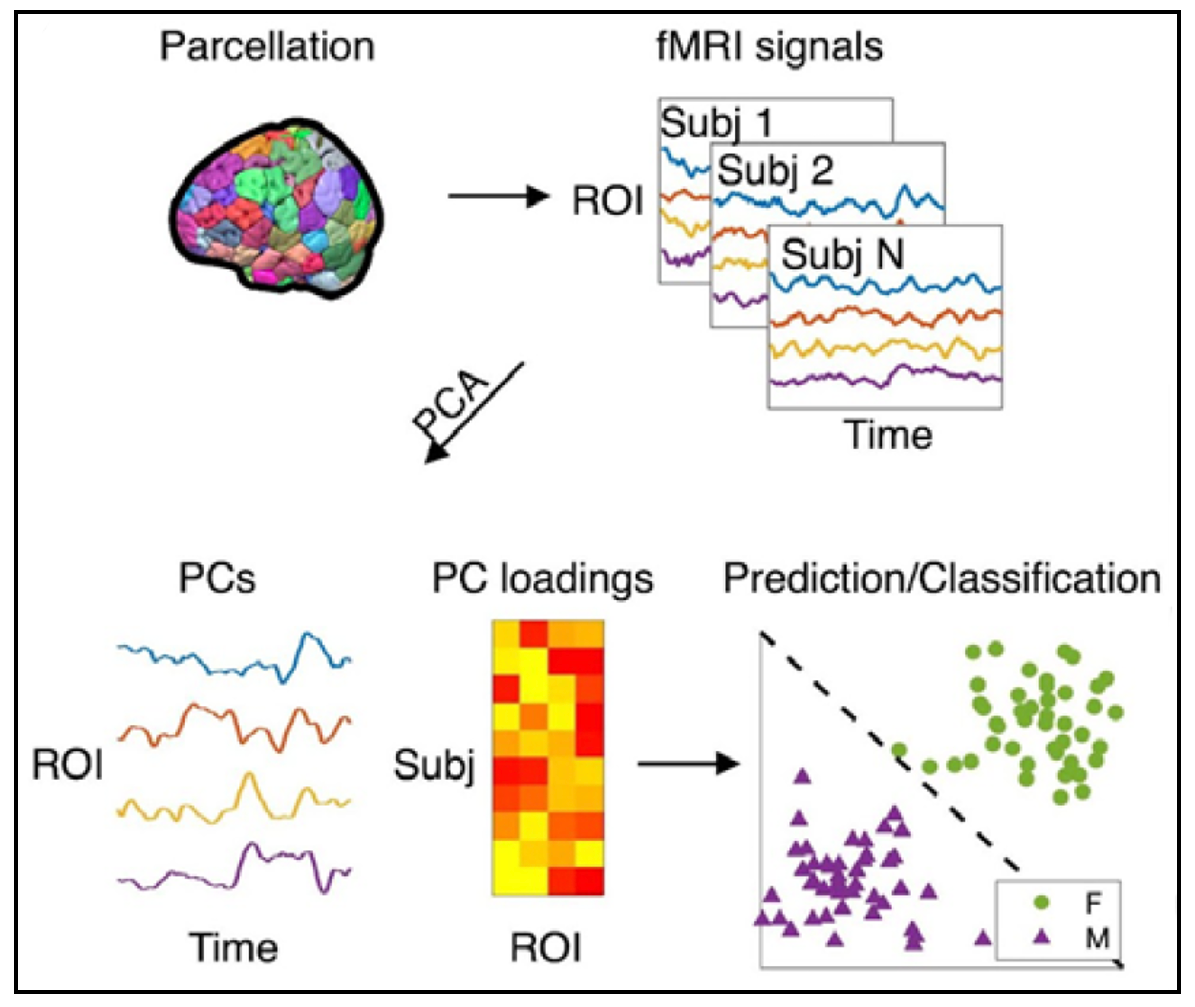
\includegraphics[width=\linewidth]{topf_neu.png}
  \caption{TOPF captures individual differ-ences in brain activity and successfully predicts phenotypes across cognition, emotion and personality.}
  \label{fig:topf}
\end{wrapfigure}
achieved up to 80\% accuracy in sex classification on single movie clips. Highly predictive regions were 
linked to emotion, language, and higher cognition. These promising findings await further validation over 
the course of the present project. Altogether, NV offers rich, time-evolving stimulation, allowing for the 
study of dynamic brain states across diverse scenarios. This method better reflects everyday cognitive and 
emotional challenges and may uncover novel sex differences in functional brain organization.
\par\vspace{-1\parskip}\noindent
Surprisingly, to our knowledge, no study has yet used NV to systematically examine sex differences. 
In a previous publication \parencite{eickhoffClinicalApplicationsMovie2020a}, we have compared the potential of movies for the study of 
individual brain differences to what running on a treadmill is to the heart during a cardiac stress-test, 
i.e. to potentially provide a standardized way to study the whole organ while it works to compare function 
across different levels of intensity and demands. In the present context, this means that NV can be expected 
to reveal sex differences in the brain that so far have been unobservable, since NV data encompass an extensive 
range of dynamic real-life situations, such as social interactions, recognition of faces or perception of 
emotions \parencite{sonkusareNaturalisticStimuliNeuroscience2019}. While isolated cognitive processes as examined in TB fMRI might not reveal 
significant sex differences, the complex interplay of these processes - as engaged during movie watching - could 
highlight more pronounced differences between women and men. This underscores the value of using naturalistic stimuli 
to uncover subtle but meaningful variations in neural processing that might be missed in more controlled, simplified 
experimental paradigms. Using careful annotations of the movies, it is also possible to identify which features 
of a given scene are particularly relevant to evoking sex differences in complex experiences and to identify 
brain networks that differ most between females and males during these experiences.\\
We aim to employ novel methodology utilizing NV paradigms to expand our understanding of sex differences in the 
brain. This approach has the potential to elucidate sex-specific neural mechanisms in response to the complex and 
dynamic content of movies and to reveal nuanced sex-specific distinctions in brain function that may not be apparent 
in more constrained experimental paradigms or everyday observations. Our methodology leverages the ecological 
validity of movie stimuli to probe complex, multimodal cognitive processes in a controlled yet naturalistic setting. 
Through advanced neuroimaging techniques and sophisticated data analysis methods, we anticipate uncovering 
subtle yet significant sex-based variations in neural activity and FC that can inform our understanding of 
broader cognitive and behavioural differences between females and males. To this aim, we will first consider 
temporally aggregated FC evoked by movies over the duration of several minutes. Subsequently, we will further 
disentangle which specific events evoke sex differences and examine differences in the brain networks caused by 
such events. Furthermore, we will examine how the brain’s response to the evolving narrative of the movies differs 
between the sexes. The project's comprehensive approach of examining temporally aggregated as well as time resolved FC, 
network dynamics and brain activity patterns provides a multi-faceted view of sex differences in the brain and, 
which can have implications for understanding sex differences in cognition, behavior, and susceptibility to certain 
neurological and psychiatric conditions.\\
Results from the proposed project have the potential to add a crucial new dimension to current knowledge on 
cognitive sex differences. Psychologically, these insights deepen our understanding of normative sex differences; 
clinically, they may help clarify why certain psychiatric and neurological disorders manifest differently in women 
and men. Such knowledge can potentially enhance diagnostic accuracy, inform personalized treatments, and support the 
development of sex-specific healthcare and education strategies.\\
Throughout the proposal, for ease of reading, the term “sex” will refer to the self-reported (biological) sex and 
appearance of the participants. At the same time, we fully acknowledge that “gender identity”, i.e. the 
subjective identification of an individual as female, male, or one of the other gender identities which might 
be also fluid, also play important roles, which however, are beyond the scope of the present project. 

\subsection*{Data: The Ju-MOVIES dataset}
The work proposed here will be based on a data set that has already been acquired and is ideally suited for 
the examination of sex differences through a NV approach. Over the course of the project, further data will be collected.
The paradigm comprises seven movie clips of about 8 - 10 minutes length, which are all excerpts from Hollywood movies 
(“Dirty Dancing”, “Scream”, “Dead Poets Society”, “Forrest Gump”, “Dead Man Walking”, “Life is Beautiful”, 
“The Good, the Bad, the Ugly”). The specific movie stimuli were chosen to cover a variety of social interactions 
and complex situations as well as multifaceted emotions evolving over the course of the movie to match 
the complex nature of real-life experiences. Considering that viewers lack the context of the entire movie, 
each stimulus was chosen to be long enough for the viewers to understand the situation, empathize with characters and 
follow the evolving narrative. Additionally, participants watch a compilation of 12 short movie clips (“Short Sequences”),
which were again taken from Hollywood movies and completed two RS scans of about 9 minutes length with their eyes open. \\
So far, we collected data of 135 healthy participants (68 males, age 18 - 35 years, mean age = 24.33 years). 
All fMRI data are acquired on a Siemens 3T Prisma scanning (Siemens, Erlangen, Germany) with a 64-channel head coil 
at the Imaging Core Facility of Research Centre Jülich, using a T2w multiband echo planar imaging sequence with the 
following parameters: repetition time (TR) = 980ms, echo time (TE) = 30ms, flip angle = 70°, field of view 
(FOV) = 207 x 207mm, voxel size=2.2 x 2.2 x 2.0mm3, number of slices: 64, multiband acceleration factor=4, 
phase encoding direction=AP,  FoV=207mm). A mirror fixed on the head coil allows participants to see a screen used 
to display the movies. In-ear headphones are used for ear protection and to deliver the movie sound. 
Additionally, a structural T1w image is acquired using an MP-RAGE sequence (TR=2000ms, TE=2.45ms, TI=900ms, 
flip angle=8°, FoV: 256mm) yielding 1mm3 voxels.\\
Saliva samples are collected from each participant and levels of cortisol, oestradiol, progesterone, and testosterone 
are analysed by a specialized laboratory. Control for fluctuating hormone levels is essential for a meaningfully 
interpretation of potential sex differences in functional brain. Furthermore, data OC intake is noted for 
female participants. To characterize the movie stimuli in more detail, emotions perceived by viewers of the movies were assessed by 
44 German participants (23 males, age 20-30 years, mean age 25.05 years) who watched all movie stimuli 
while simultaneously rating six basic emotions 
\begin{wrapfigure}{r}{0.3\textwidth} % r = rechts, l = links
  \vspace{-10pt} % optional: kleine Korrektur, damit es bündig startet
  \includegraphics[width=\linewidth]{emotions_DMW_edited.png}
  \caption{Exemplary emotion annotation for one of the movie stimuli..}
  \label{fig:dmw}
\end{wrapfigure}
(happiness, fear, surprise, sadness, disgust and anger \parencite{ekmanConstantsCulturesFace1971a}). 
Rating were collected by the ReMoTa toolbox (Real-time Movie Tagging v0.0; \parencite{lettieriEmotionotopyHumanRight2019a}). 
Participants watched the movies on a laptop and rated their feelings by use of the keyboard. 
All emotions were rated simultaneously on a scale from 0 to 100 at a sampling rate of 10hz. 
The emotion ratings confirmed the multifaceted and diverse emotions elicited by the 
different movie stimuli. In a further annotation, two independent raters quantified the following 
features: faces, bodies, male / female presenting characters, ethnicity of characters, presence of children, 
adults, crowds, hands, buildings, vehicles, food, landscapes, animals, plants, movement, social interactions, 
place (inside or outside / urban vs. non-urban), time of day (day or night), weather, presence of music and 
camera movements.

\subsection*{Work Program and Research Methods}
The overarching goal of the proposed project is to complement existing research on sex differences by employing a 
NV approach. This method promises new insights into sex differences in the brain response to complex and 
dynamically evolving situations akin to what the brain has to deal with in real life. 
Results can go beyond existing studies based on both TB or RS approaches and promise novel insights that 
could so far not be achieved with existing research approaches. Specifically, we will examine which types 
of complex situations as depicted in the movie stimuli result in most pronounced sex differences. 
In the next steps, we will further disentangle which events within the movies' narrative drive these sex 
differences and examine how females’ and males’ brains respond differentially to the evolving narrative of the movies. 
We expect this novel approach to the study of cognitive sex differences together with the project's comprehensive 
approach of examining temporally aggregated FC, event-related responses, network dynamics and brain 
activity as well as hormone related variability to provide important new insights into the 
multi-faceted spectrum of sex differences of the brain in action.\\ 
Firstly, in work package (WP) 1 we aim to go beyond existing results on sex differences in the RS 
by examining sustained FC over the course of a variety of movies of several minutes length. Using a temporally 
aggregated FC approach as commonly used for RS data, results of this WP will identify sex differences in 
“action brain states” and their underlying brain networks.\\ 
In WP 2, we will then employ a time resolved FC approach to identify temporally specific events driving sex 
differences in the experience of complex situations. This approach makes use of the know dynamics and content 
of the movies. Detailed annotations of the movie content will be used to characterize the type of situations 
that drive sex differences together with revealing sex specific cognitive strategies when encountering such situations.\\ 
In WP3, rather than looking at temporally aggregated or time resolved FC patterns we will examine the brain 
activation invoked by the movies. In particular, we will extract (within each brain region) typical 
female and male brain responses to the dynamically evolving movie content. This approach complements 
results from WP1 and WP2 through an understanding of how females' and males' brains respond differentially 
to the evolving narrative of the movies. 

\subsection*{WP 1: The Brain in Action - The Naturalistic Viewing Action State (NV-AS) }
Several studies have shown that sex classification based on RS FC can achieve high classification accuracies 
\parencite{casanovaCombiningGraphMachine2012a,ritchieSexDifferencesAdult2018, weisSexClassificationResting2020a,wierschAccurateSexPrediction2023a,wierschSexDifferencesBrain2021a} 
by capturing temporally aggregated FC patterns evoked over a sustained state of free thought or mind wandering. 
Since these RS brain patterns are independent of any external stimulation, they are often taken as a proxy 
for intrinsic brain organization, and in that sense, constitute more of a trait rather than an actual state.\\ 
The present WP aims to supplement existing results on sex differences in the brain by examining temporally 
aggregated FC patterns induced by the complex narratives presented in the movies. In contrast to RS, 
we expect movie induced brain patterns to represent states that are strongly dependent on the content of the movies. 
As this content is known, it can be used to characterize evoked FC patterns and sex differences between them. 
Thus, in this WP we will consider sustained brain “action states” (ASs) evoked by different movies and 
ompare sex classification accuracies based on different naturalistic viewing ASs (NV-ASs) to RS. 
Since sex differences in NV-ASs depend on movie content, annotations the content will be employed to 
characterize the evoked brain NS-ASs and sex differences between them. 
Thus, this WP will provide insights 
into which kind of situations evoke particularly prominent differences between females and males. Here, we are 
looking at sex differences in the overall experience of complex situations, which is different both from TB 
studies looking at sex differences within specific cognitive tasks and from RS which mostly reflects intrinsic 
brain organization. We assume, that putting the brain into action while experiencing different complex situations 
should bring out differences between females and males more strongly than unrestricted and thus uncontrolled 
free thought can \parencite{vanderwalIndividualDifferencesFunctional2017}.\\
To compare enduring NV-AS to RS and amongst different movies, we will employ a similar approach as 
in our previous work \parencite{weisSexClassificationResting2020a}.\\ 
Briefly, after parcellating the fMRI data into non-overlapping parcels based on an established parcellation 
(e.g. \parencite{schaeferLocalGlobalParcellationHuman2018}), 
a mean activation time course will be computed for each parcel and correlated with those of each of the other parcels. 
Then, for each parcel individually, the FC pattern with the rest of the brain will be used as features 
to train a sex classifier for which classification accuracy will be determined by use of a cross validation (CV) 
approach. This procedure results in a spatial map of sex classification accuracies across the brain for RS and each 
NV-AS (i.e. each movie). Importantly, and in contrast to the majority of previous studies, 
we will include hormone levels and OC status in women as confounds into all prediction analyses in WP1 to 
ensure that results delineate actual differences between the sexes, rather than hormone related variability. 
In doing so, we will take particular care to control for confound leakage \parencite{hamdanConfoundleakageConfoundRemoval2022a}, 
which might bias results of the prediction analyses. 
\subsubsection*{WP 1.1:  Comparing sex classification accuracies between RS and NV-ASs}
As a first step, within each parcel, sex classification performance (across CV folds) will be compared between RS and 
NV-AS (averaged across all movies) by use of corrected resampled t-tests \parencite{nadeauInferenceGeneralizationError2003a}. 
Higher classification accuracies during NV (compared to RS) will reveal cognitive sex differences 
that are specific to the brain in action rather than to its intrinsic organization. In addition, the spatial distribution of 
highly discriminative parcels in NV will highlight the brain networks underlying these sex differences in the NV-AS. Cognitive domains 
related to the identified brain networks can be characterized by use of functional decoding \parencite{foxMetaanalysisHumanNeuroimaging2014a}. 
While sex differences 
have often been reported in the DMN for RS \parencite{weisSexClassificationResting2020a,zhangFunctionalConnectivityPredicts2018}, 
for NV-AS, we expect sex differences in higher 
cognitive or task-general networks \parencite{hugdahlExistenceGeneralizedNonspecific2015a}. Furthermore, we expect sex classification 
based on NV-AS to outperform RS, as similar effects have been observed for other phenotypes 
\parencite{finnCanBrainState2017a,vanderwalIndividualDifferencesFunctional2017} and NV has been shown to increases individual 
identifiability over RS \parencite{krollNaturalisticViewingIncreases2023}. 

**** bis hier

\subsubsection*{WP 1.2: Which movie features drive sex classification accuracies?}
To further examine which kinds of complex situations maximize sex differences in the brain, we will characterize each movie 
clip by several visual and auditory features across the duration of the movie clips. These will comprise low-level features like mean 
motion energy, visual brightness and auditory loudness, high-level features like number of faces, social interactions and words, 
which can be automatically extracted (Mcnamara, et al. 2017; Radford, et al. 2023), 
and further movie features that have been acquired in Ju-MOVIE-An. We will then compare sex classification accuracies 
across the whole brain between the eight different movies clips by use of a multiple regression approach, which will 
delineate which movie features drive classification performance for each brain parcel. 
As higher classification performance indicates more pronounced differences between the sexes, this procedure will 
result in a “movie feature profile” explaining which features of the movies result in most pronounced sex differences. 
By clustering brain parcels according to their movie feature profiles, we will identify brain networks in which sex 
differences are conjointly driven by specific features of the movies. We hypothesize that certain brain 
networks will comprise specific cognitive domains, in particular those that have been identified in 
classical group studies, which identified sex differences in cognitive domains like language and spatial cognition (Halpern 2000; Kimura 2000). Other networks can be expected to comprise more generalized and non-specific cognitive resources which are independent of the specific situation (Hugdahl, et al. 2015). We expect domain-specific brain networks to overall achieve higher sex classification accuracies than domain-general networks.
In an exploratory approach, we will compare the expressions of these networks in females and males by 
computing the first principal component of network FC patterns in females and males separately, 
thus identifying the “typical” female and male brain network pattern for each movie feature cluster. An exploration of these sex specific movie feature networks should help elucidate sex specific cognitive strategies in response to complex life-like situations. 
Main Goal: Characterize sex differences in the NV-AS to reveal situationally modulated sex differences 
that may not be evident in RS.
Open Question: Will sex specific movie feature networks differ systematically, 
and what do these differences suggest about sex-specific cognitive strategies?



\printbibliography

\end{document}
